\documentclass[11pt,a4paper,oneside]{article}
\usepackage[a4paper,top=2cm,bottom=2.5cm,left=2.5cm,right=2cm]{geometry}
\usepackage[T1]{fontenc}
\usepackage[utf8]{inputenc}
\usepackage[english]{babel}
%\usepackage{frontespizio}
\usepackage{graphicx}
\usepackage{subfig}
\usepackage[english]{varioref}

\begin{document}

%opzione per doppio interlinea
\baselineskip 22pt


%Indice%
\tableofcontents\thispagestyle{empty}\clearpage

\section{Introduction}
\pagenumbering{arabic}
\baselineskip 12pt

\section{The dataset}


\section{Task 1: Related works}



\section{Task 2: Scratch CNN}
We developed different models of neural networks to work with the given dataset from scratch and we did different test to find the better hyperparameters to build the final model. This section is divided in three parts: in the first one we describe the main preprocessing applied to the data before the training of the models. Then we show how we built a model for classifying the dataset images between \textit{mass} abnormality and \textit{calfication} abnormality. In the last part, we describe the model built to classify between \textit{benign} and \textit{malignant} abnormality.

\subsection{Data Preprocessing}
Starting from the numpy arrays of the dataset images we were given, first of all we deleted all the samples associated with the \textit{baseline patch} label. Since this labeled images were placed in the even positions of the dataset, we just selected all the odd-index samples al discard the others. This is done both for the training data and the test data. \\
Then we aggregated the labels according to the classification that we needed to do: in the $Task\ 2.1$ the classes \textit{mass benign} and  \textit{mass malignant} were aggregated in a unique class \textit{mass}, and so for the \textit{calcification} classes. On the other hand, in the $Task\ 2.2$ we aggregated  \textit{mass benign} and  \textit{cacification benign} in the \textit{benign} class, and the other labels in the \textit{malignant} class.

\begin{figure}[htbp]
\centering
	\subfloat[][$Task\ 2.1$: 0 for \textit{mass}, 1 for \textit{calcification} \label{fig:label_mass_calc}]
		{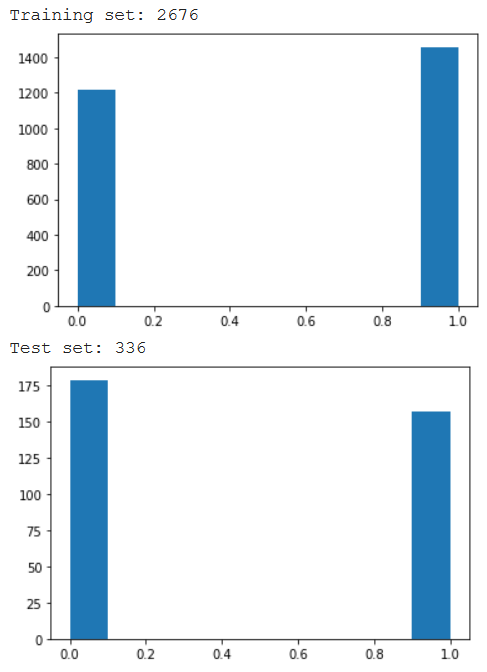
\includegraphics[width=.4\textwidth]{images/label_mass_calc}} \quad
	\subfloat[][$Task\ 2.2$: 0 for \textit{benign}, 1 for \textit{malignant} \label{fig:label_benign_malign}]
		{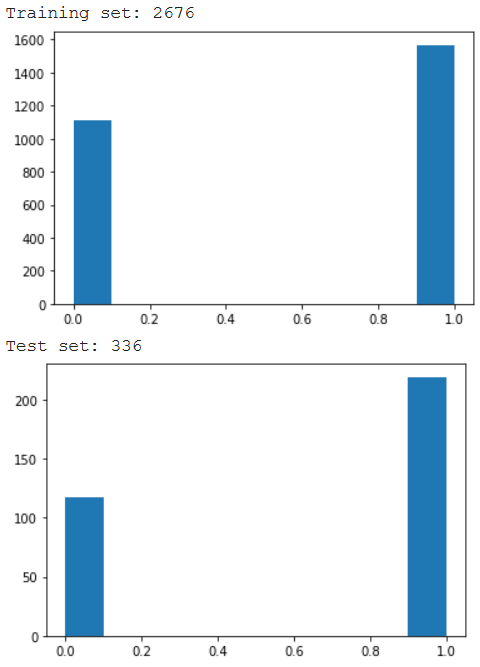
\includegraphics[width=.4\textwidth]{images/label_benign_malign}} \\
\caption{Label distribution}
\label{fig:label distribution}
\end{figure}

For the first case, we can see from the figure that the labels are pretty much equally distributed. Instead, in the second case the dataset is a little more unbalanced towards the \textit{benign} class.

\subsection{Task 2.1}
For the first classification, we first tried to build a simple CNN 

\begin{verbatim}

\end{verbatim}

\subsection{Task 2.2}


\section{Task 3: Pretrained network}


\section{Task 4: Baseline patches}


\section{Task 5: Ensemble network}

\end{document}
